\documentclass[11pt,a4paper]{article}

% package importing
%\usepackage[margin=2cm]{geometry}
\usepackage{geometry}
 \geometry{
 a4paper,
 %total={170mm,257mm},
 left=20mm,
 top=20mm,
 right=20mm,
 bottom=20mm,
 }
 		%$$$$$$ fonts settings $$$$$$%
%\usepackage[sc]{mathpazo}  %for palatino font
%\usepackage{eulervm}  %for Euler maths font

		%$$$$$$ package imports $$$$$$%
\usepackage{amsmath}  %for mathematics
\usepackage{titlesec}  %for title spacing only
\usepackage{lipsum}  %random huge text generation
\usepackage{titlesec} %for changing font of titles 
\usepackage{amssymb}  %for real number set symbol
\usepackage{amsthm}  %for mathematics package
\usepackage{mathtools}  %for floor and ceiling
\usepackage{algorithmicx}  %for dynamic algorithm
\usepackage{algorithm}  %algorithm micro
\usepackage{algpseudocode}  %pseudocode commands
\usepackage{wrapfig}  %for wrapping figures around text
\usepackage{multicol}  %for multiple columns floats
\usepackage{enumitem}  %for enumerate numbering
\usepackage{url}   %for writing the url
\usepackage{color}  %for colorred text
\usepackage{tcolorbox}  %for colour box highlighting
\usepackage{listings}  %for code listing

% $$$$$$$$$ new command and theorems self-defined
\theoremstyle{definition}
\newtheorem{theorem}{Theorem}[section]
\newtheorem{corollary}{Corollary}[theorem]
\newtheorem{lemma}[theorem]{Lemma}
\newtheorem*{remark}{Remark}
\newtheorem{definition}{Definition}[section]
\newtheorem{example}{Example}[section]
\newtheorem{notation}{Notation}[section]
\newtheorem{algoalgorithm}{Algorithm}[section]
\newtheorem{method}{Method}[section]

% $$$$$$$$ set general info $$$$$$$
\title{\textsl{National University of Singapore} \\ \textbf{CS2106 Operating System}\\ Second Half Summary Notes}
\author{\textit{Dong Shaocong} A0148008J}

% $$$$$$$$ package parameter setting $$$$$$$$$

% for title spacing {left}{before}{after}  ----------------------------
\titlespacing\section{0.5pt}{10pt plus 2pt minus 2pt}{2pt plus 2pt minus 1pt}
\titlespacing\subsection{0.5pt}{10pt plus 2pt minus 2pt}{2pt plus 2pt minus 1pt}
\titlespacing\subsubsection{0.5pt}{10pt plus 2pt minus 2pt}{2pt plus 2pt minus 1pt}

% for title font specifications  ------------------------------------------
\titleformat{\section}
  {\normalfont\fontsize{16}{16}\bfseries}
  {\thesection}{1em}{}
  
\titleformat{\subsection}
  {\normalfont\fontsize{14}{14}\bfseries}{\thesection}{1em}{}
  
\titleformat{\subsubsection}
  {\normalfont\fontsize{13}{13}\bfseries}{\thesection}{1em}{}

% declare floor and ceiling functions   ------------------------------------------
\DeclarePairedDelimiter\ceil{\lceil}{\rceil}
\DeclarePairedDelimiter\floor{\lfloor}{\rfloor}

% set the numbering of enumerate to numbers------------------------------------------
\setlist[enumerate]{label*=\arabic*.}
%\setlist{nolistsep}
\newenvironment{myitemize}
{ \begin{itemize}
    \setlength{\itemsep}{5pt}
    \setlength{\parskip}{0pt}
    \setlength{\parsep}{0pt}     }
{ \end{itemize}                  } 
\newenvironment{myenumerate}
{ \begin{enumerate}
    \setlength{\itemsep}{5pt}
    \setlength{\parskip}{0pt}
    \setlength{\parsep}{0pt}     }
{ \end{enumerate}                } 

% $$$$$$$$$ math symbols cheatsheet
% Caligraphic letters: $\mathcal{A}$ 
% Mathbb letters: $\mathbb{A}$
% Mathfrak letters: $\mathfrak{A}$ 
% Math Sans serif letters: $\mathsf{A}$ 
% $$$$$ color text commands ------------
\newcommand{\redtt}[1]{{\color{red}\texttt{#1}}}
\newcommand{\bluett}[1]{{\color{blue}\texttt{#1}}}
\newcommand{\browntt}[1]{{\color{brown}\texttt{#1}}}
\newcommand{\bluebf}[1]{{\color{blue} \huge \textbf{#1}}}
\renewcommand{\emph}[2]{\redtt{#1} \bluebf{#2}}
%-------------------------------------------------------

% $$$$$$$$ start of documents $$$$$$$$$
\begin{document}
\maketitle
\section{Memory Management}

\begin{definition}{\textbf{Memory \& OS responsibility}}
	\begin{myitemize}
		\item \textbf{Memory} used to store: kernel code and data; user code and data
		\item \textbf{OS Responsibilities}: 
		\begin{myitemize}
			\item Allocate memory to new processes.
			\item Manage process memory.
			\item Manage kernel memory for its own use.
			\item Provide OS services to: get more memory, free memory, protect memory
		\end{myitemize}
	\end{myitemize}
\end{definition}

\begin{definition}{\textbf{Physical Memory Organization}}
	\begin{myitemize}
		\item The actual matrix of capacitors (DRAM) or flip-flops (SRAM) that stores data and instructions.
		\item Arranged as an array of bytes.
		\item Memory addresses serve as byte indices.
	\end{myitemize}
\end{definition}

\begin{definition}{\textbf{Word}}: CPU data transfer unit
	\begin{myitemize}
		\item 1 byte in 8-bit machines (ATMega328P, Intel 8080), 2 bytes in 16 bit machines (Intel 80286),  4 bytes in 32-bit machines (Intel Xeon), 8 bytes in 64-bit machines (Intel Celeron)
	\end{myitemize}
\end{definition}

\begin{minipage}{0.6\linewidth}
	\begin{definition}{\textbf{Endianness}}
	\begin{center}
		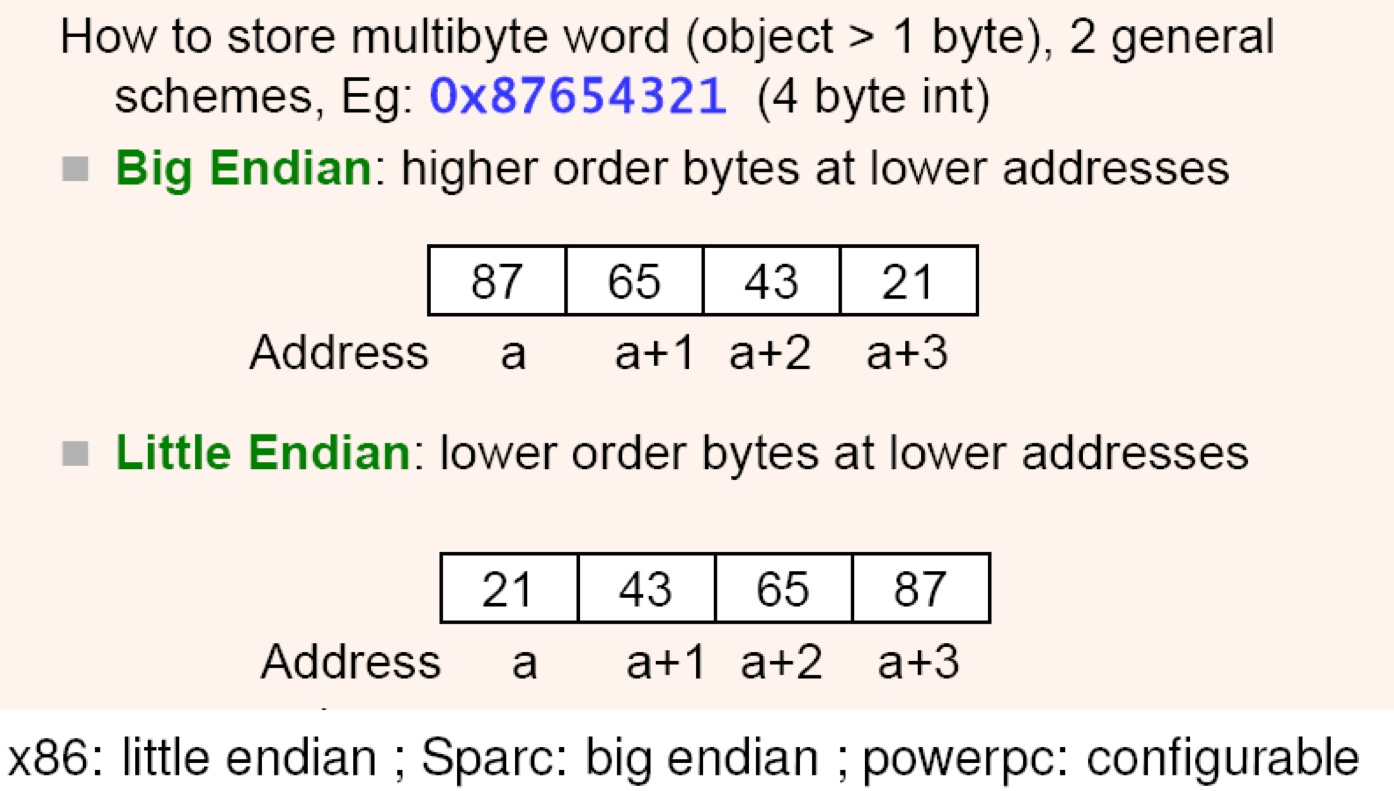
\includegraphics[width=1\linewidth]{m4/endianness}
	\end{center}
\end{definition}
\end{minipage}
\begin{minipage}{0.40\linewidth}
	\begin{definition}{\textbf{Alignment Issues}}
	\begin{center}
		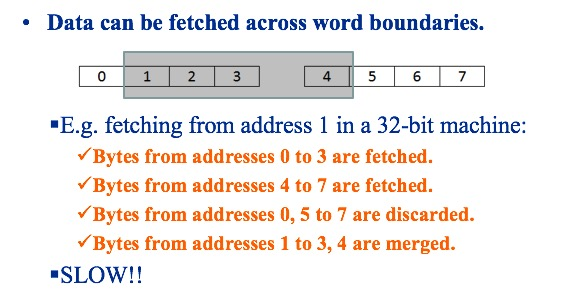
\includegraphics[width=1\linewidth]{m4/alignmentIssues}
	\end{center}
	
	Add unused bytes to ensure data structures always in units of words. Instructions fetched across word boundaries trigger ``Bus Error'' faults.
\end{definition}
\end{minipage}

\begin{tcolorbox}
	\textsf{Why Memory Management?}
	\begin{myitemize}
		\item We want to use memory efficiently
		\item We want to protect processes from each other
	\end{myitemize}
\end{tcolorbox}

\begin{minipage}{0.4\linewidth}
	\begin{myitemize}
		\item \textbf{Logical addresses}: These are the addresses as “seen” by executing processes code.
		\item \textbf{Physical addresses}: These are addresses that are actually sent to memory to retrieve data or instructions.
	\end{myitemize}
\end{minipage}
\begin{minipage}{0.6\linewidth}
	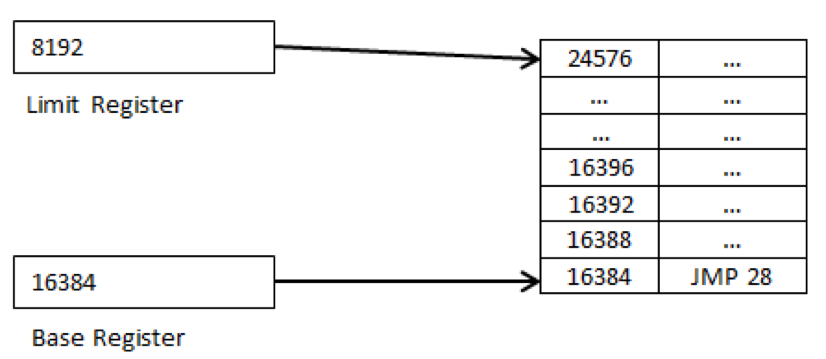
\includegraphics[width=\linewidth]{m4/logicalAddress}
\end{minipage}

\noindent \textbf{Note}: \textbf{Having multiple processes complicates memory management}:
\begin{myitemize}
	\item \textbf{Conflicting addresses}: What if $>1$ program expects to load at the same place in memory?
	\item \textbf{Access violations}: What if 1 program overwrites the code/data of another? Worse, what if 1 program overwrites parts of the operating system?
	\item The ideal situation would be to give each program a section of memory to work with. Basically each program will have its own address space!
\end{myitemize}
\textbf{To do this we require extra hardware support}:
\begin{myitemize}
	\item \textbf{Base register}: This contains the starting address for the program. All program addresses are computed relative to this register.
	\item \textbf{Limit register}: This contains the length of the memory segment.
\end{myitemize}
\textbf{These registers solve both problems}:
\begin{myitemize}
	\item We can resolve address conflicts by setting different values in the base register.
	\item If a program tries to access memory below the base register value or above the (base+limit) register value, a ``segmentation fault'' occurs!
	\item All memory references in the program are relative to the Base Register. E.g. ``jmp 28'' above will cause a jump to location 16412.
	\item Any memory access to location 24576 and above (or 16383 and below) will cause segmentation faults. (Other programs will occupy spaces above and below the segment given to the program shown here.)
	\item Base and limit registers allow us to partition memory for each running process: Each process has its own fixed partition, assuming that we know how much memory each process needs.

\end{myitemize}

\begin{definition}{\textbf{Fragmentation Issues}}
	
\begin{minipage}{0.7\linewidth}
	\begin{myitemize}
		\item \textbf{Internal fragmentation}:
		\begin{myitemize}
			\item Partition is much larger than is needed.
			\item Cannot be used by other processes.
			\item Extra space is wasted.
		\end{myitemize}
		\item \textbf{External fragmentation}:
		\begin{myitemize}
			\item Free memory is broken into small chunks by allocated memory.
			\item Sufficient free memory in TOTAL, but individual chunks insufficient to fulfil requests.
		\end{myitemize}
	\end{myitemize}
\end{minipage}
\begin{minipage}{0.3\linewidth}
	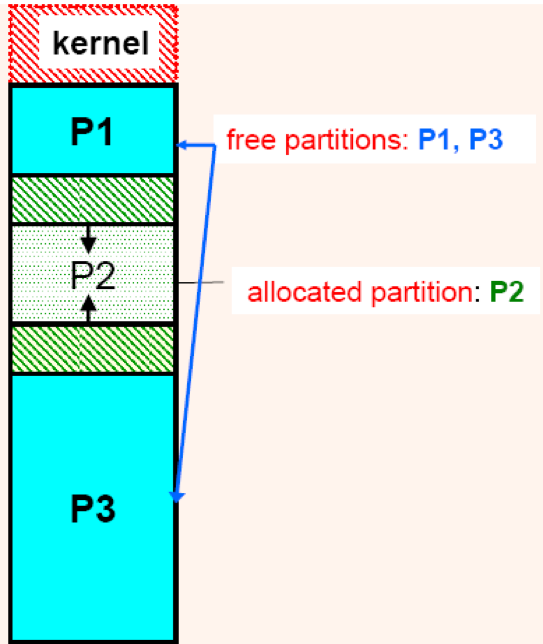
\includegraphics[width=0.8\linewidth]{m4/fragmentationIssues}
\end{minipage}
\end{definition}

\begin{definition}{\textbf{Managing Memory within processes}}
	OS allocates memory for instructions. Global variables are created as part of the program’s environment, and don’t need to be specially managed. A \textbf{``stack''} is used to create local variables and store local addresses. A \textbf{``heap''} is used to create dynamic variables.
	
\begin{minipage}{0.55\linewidth}
	E.g. in UNIX, process space is divided into:
	\begin{myitemize}
		\item \textbf{Text segments}: Read-only, contains code. May have >1 text segments.
		\item \textbf{Initialised Data}: Global data initialized from executable file. E.g. when you do: 

		char *msg[]=``Hello world!'';
		\item \textbf{BSS Segment}: Contains uninitialized globals.
		\item \textbf{Stack}: Contains statically allocated local variables and arguments to functions, as well as return addresses.
		\item \textbf{Heap}: Contains dynamically allocated memory.
	\end{myitemize}
\end{minipage}
\begin{minipage}{0.45\linewidth}
	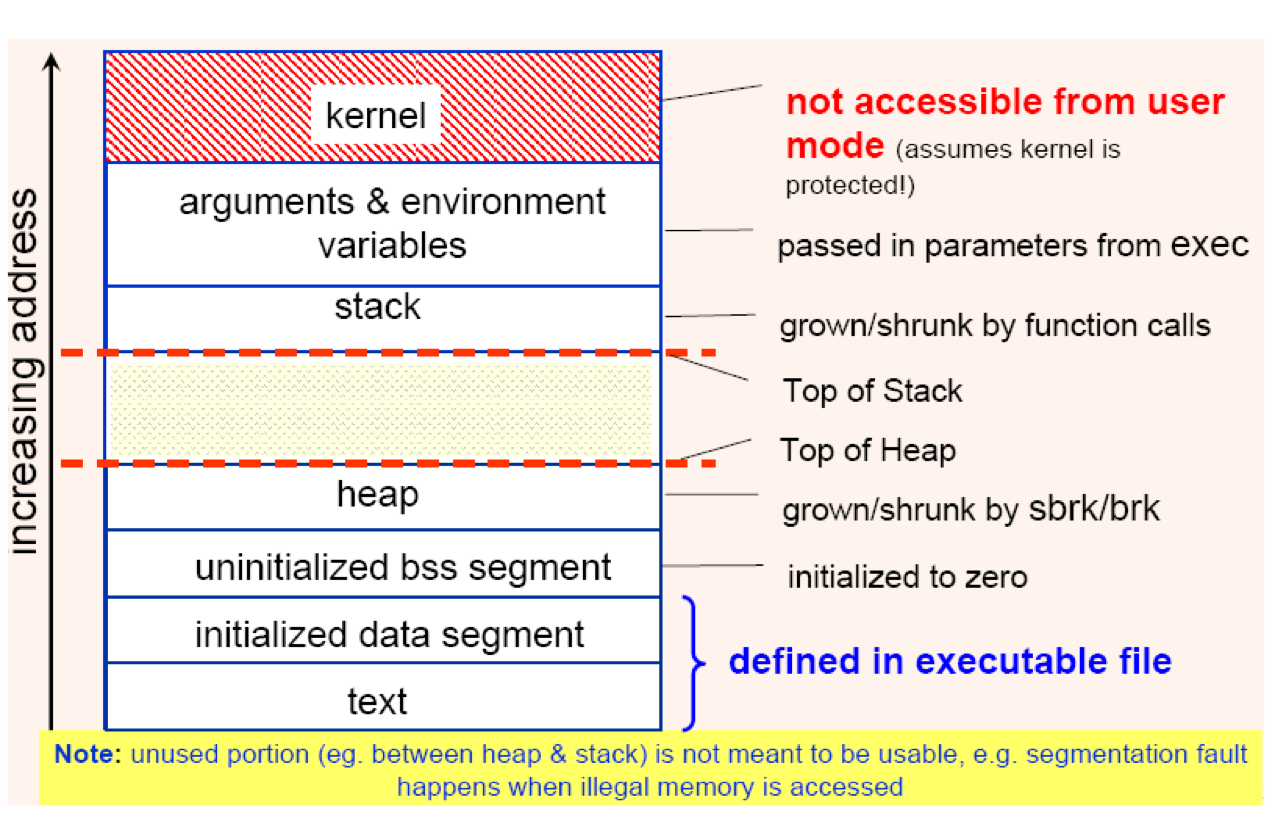
\includegraphics[width=\linewidth]{m4/processMemory}
\end{minipage}

\end{definition}

\begin{definition}{\textbf{Managing Free Memory}}
	
\begin{minipage}{0.5\linewidth}
Memory is divided up into fixed sized chunks called \textbf{``allocation units''}. Common sizes range from several bytes (e.g. 16 bytes) to several kilobytes,(a).
\begin{myitemize}
	\item \textbf{Bit maps}
	\item \textbf{Free/Allocated List}
\end{myitemize}
	
\end{minipage}
\begin{minipage}{0.5\linewidth}
	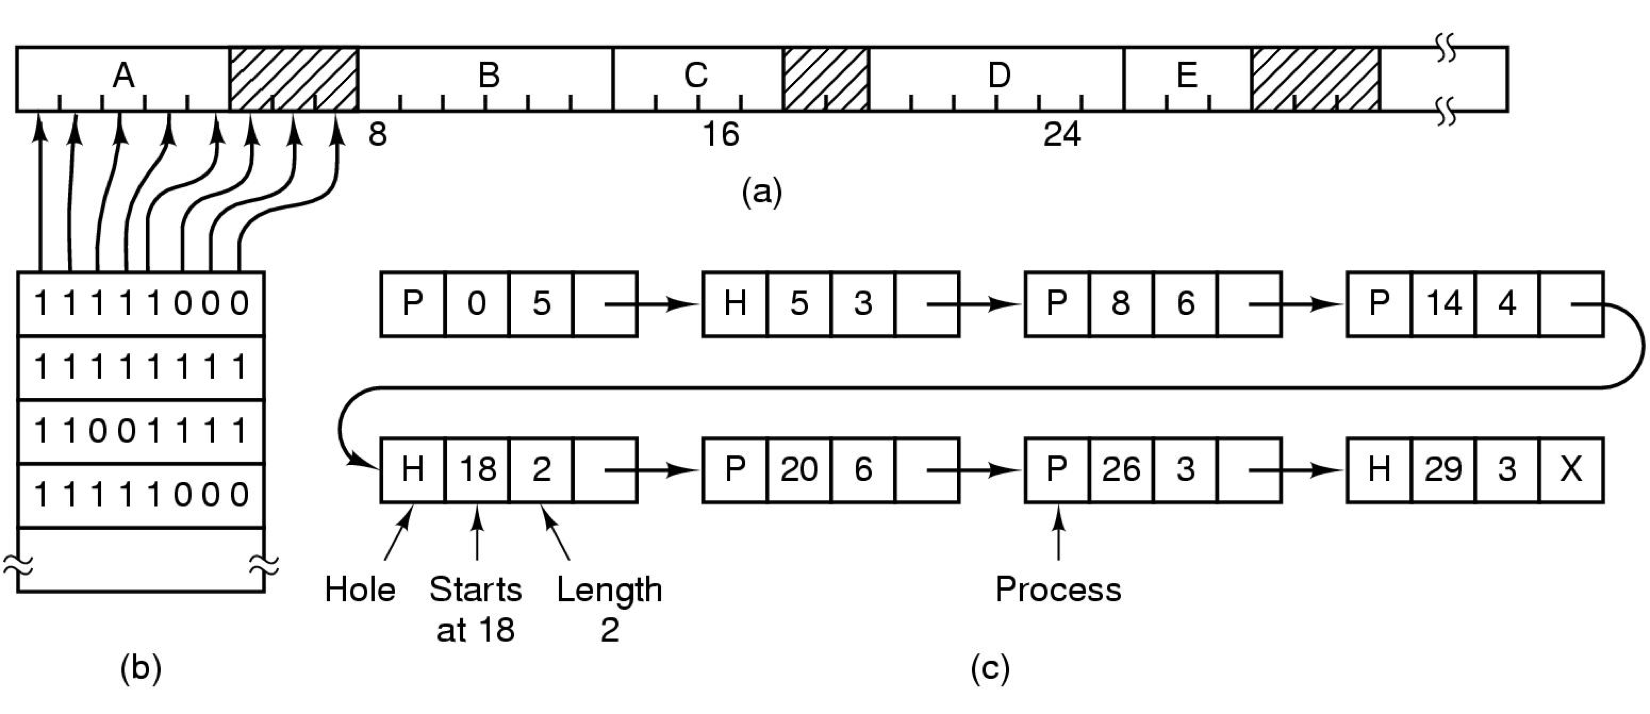
\includegraphics[width=\linewidth]{m4/freeMemoryManagement}
\end{minipage}

\noindent\textbf{Bit Map (b)}
\begin{myitemize}
	\item Each bit corresponds to an allocation unit. A ``0'' indicates a free unit, a ``1'' indicates an allocated unit.
	\item If a program requests for 128 bytes:
	\begin{myenumerate}
		\item Find how many allocation units are needed. E.g. if each unit is 16 bytes, this corresponds to 8 units.
		\item Scan through the list to find 8 consecutive 0's.
		\item Allocate the memory found, and change the 0's to 1's.
	\end{myenumerate}
	\item If a program frees 64 bytes: Mark the bits corresponding to the 4 allocation units as ``0''.

\end{myitemize}

\noindent\textbf{Linked list (c)}
\begin{myitemize}
	\item A single linked list is used to track allocated (``P'') units and free (``H'') units. Each node on the linked list also maintains where the block of free units start, and how many consecutive free units are present in that block.
	\item Allocating free memory becomes simple: Scan the list until we reach a ``H'' node that points to a block of a sufficient number of free units.
	\vspace{2mm}
	
	\begin{minipage}{0.5\linewidth}
		\begin{myitemize}
			\item The list is implemented as a double-linked list.
			\begin{myitemize}
				\item Diagram below shows possible ``neighbor combinations'' that can occur when a process X terminates.
				\item The ``back pointer'' in a double-linked list makes it easy to coalesce freed blocks together.
			\end{myitemize}
		\end{myitemize}
	\end{minipage}
	\begin{minipage}{0.5\linewidth}
		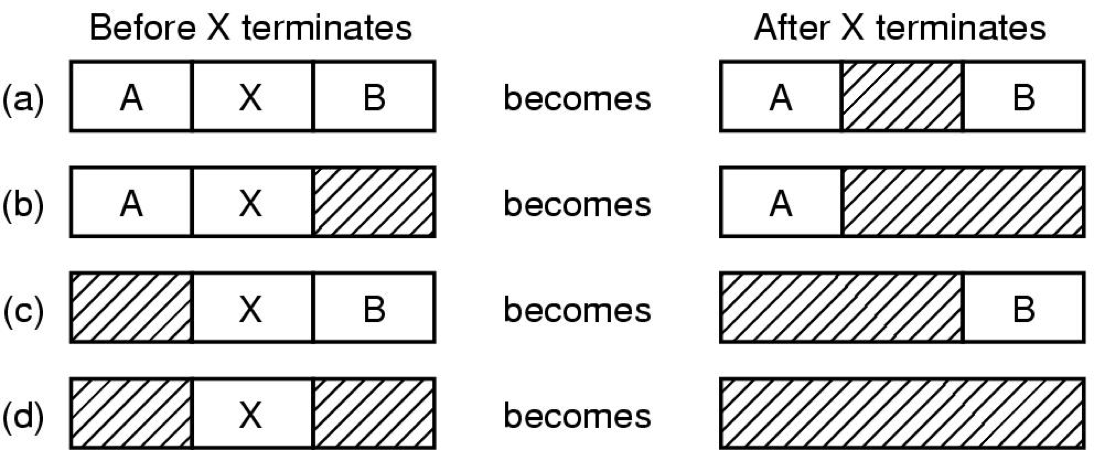
\includegraphics[width=\linewidth]{m4/freeLinkedList}
	\end{minipage}
\end{myitemize}
\end{definition}

\newpage
\begin{definition}{\textbf{Allocation Policies}}
	\begin{myitemize}
		\item \textbf{First Fit}:
		\begin{myitemize}
			\item Scan through the list/bit map and find the first block of free units that can fit the requested size.
			\item Fast, easy to implement.
		\end{myitemize}
		\item \textbf{Best Fit}:
		\begin{myitemize}
			\item Scan through the list/bit map to find the smallest block of free units that can fit the requested size.
			\item Theoretically should minimise ``waste''.
			\item However can lead to scattered bits of tiny useless holes.
		\end{myitemize}
		\item \textbf{Worst Fit}:
		\begin{myitemize}
			\item Find the largest block of free memory.
			\item Theoretically should reduce the number of tiny useless holes.
		\end{myitemize}
		\item \textbf{Note}: We can sort the free memory from smallest to largest for best fit (worst case unchanged), or largest to smallest for worst fit. This minimises search time. However coalescing free neighbours will be much harder.
		
		\begin{minipage}{0.4\linewidth}
		\textbf{Quick Fit: Buddy Allocation, Binary splitting}
		\begin{myitemize}
			\item Half of the block is allocated.
			\item The two halves are called ``buddy blocks''.
			\item Can coalesce again when two buddy blocks are free.
		\end{myitemize}
		\end{minipage}\hspace{5mm}
		\begin{minipage}{0.55\linewidth}
			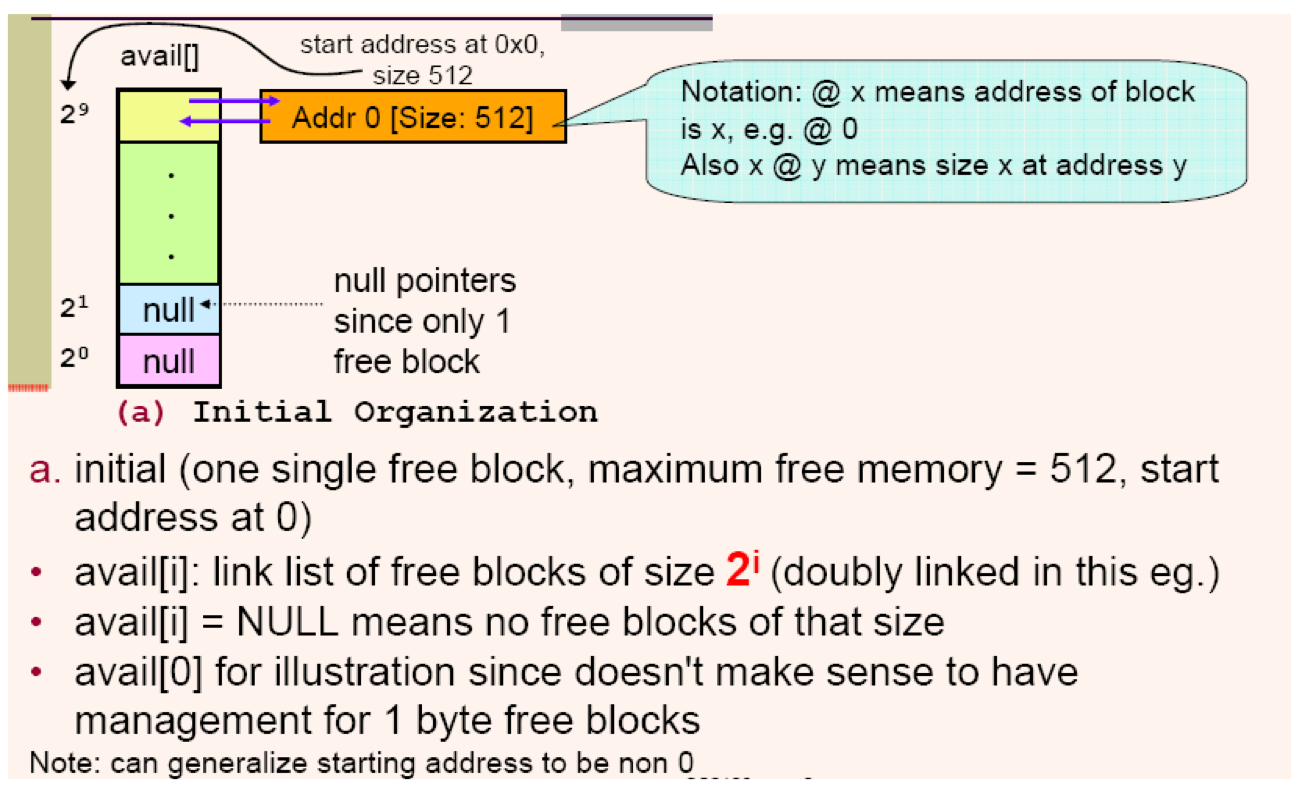
\includegraphics[width=\linewidth]{m4/buddyAllocation1}
		\end{minipage}

	\end{myitemize}
\end{definition}

\begin{example}{\textbf{Buddy Allocation}}

\begin{minipage}{0.3\linewidth}
	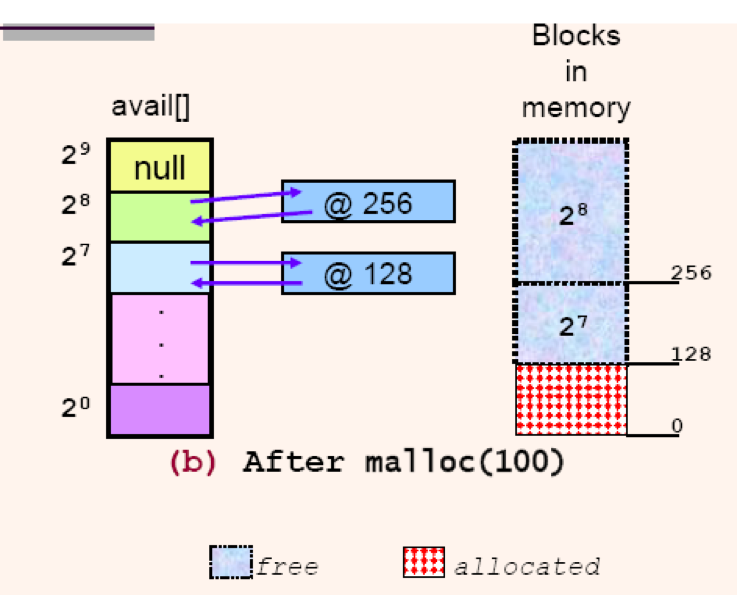
\includegraphics[width=\linewidth]{m4/buddyAllocation2}
\end{minipage}
\begin{minipage}{0.3\linewidth}
	\textsf{malloc(100)}
	
	\begin{myenumerate}
		\item Split 512 byte block into 2 blocks of 256 bytes.
		\item Split one 256 byte block into two 128 byte blocks.
	\end{myenumerate}
	
	\textsf{free(0)}: block Coalesces
\end{minipage}
\begin{minipage}{0.3\linewidth}
	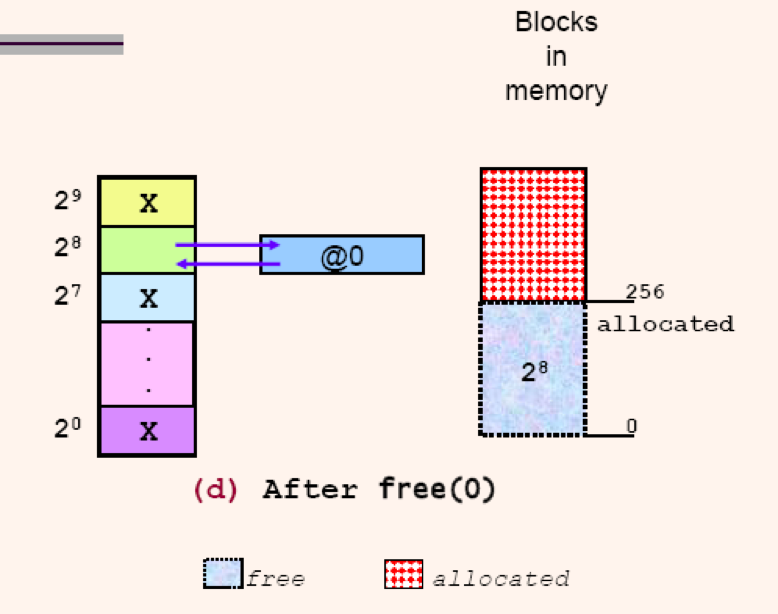
\includegraphics[width=\linewidth]{m4/buddyAllocation3}
\end{minipage}

	
\end{example}















% $$$$$$$$$$$$$$$$$$$$$$$$$$$$$$$$$$ %
\end{document}